\appendix

\chapter{Model predictions}

\begin{figure}[!htb]
    \centering
    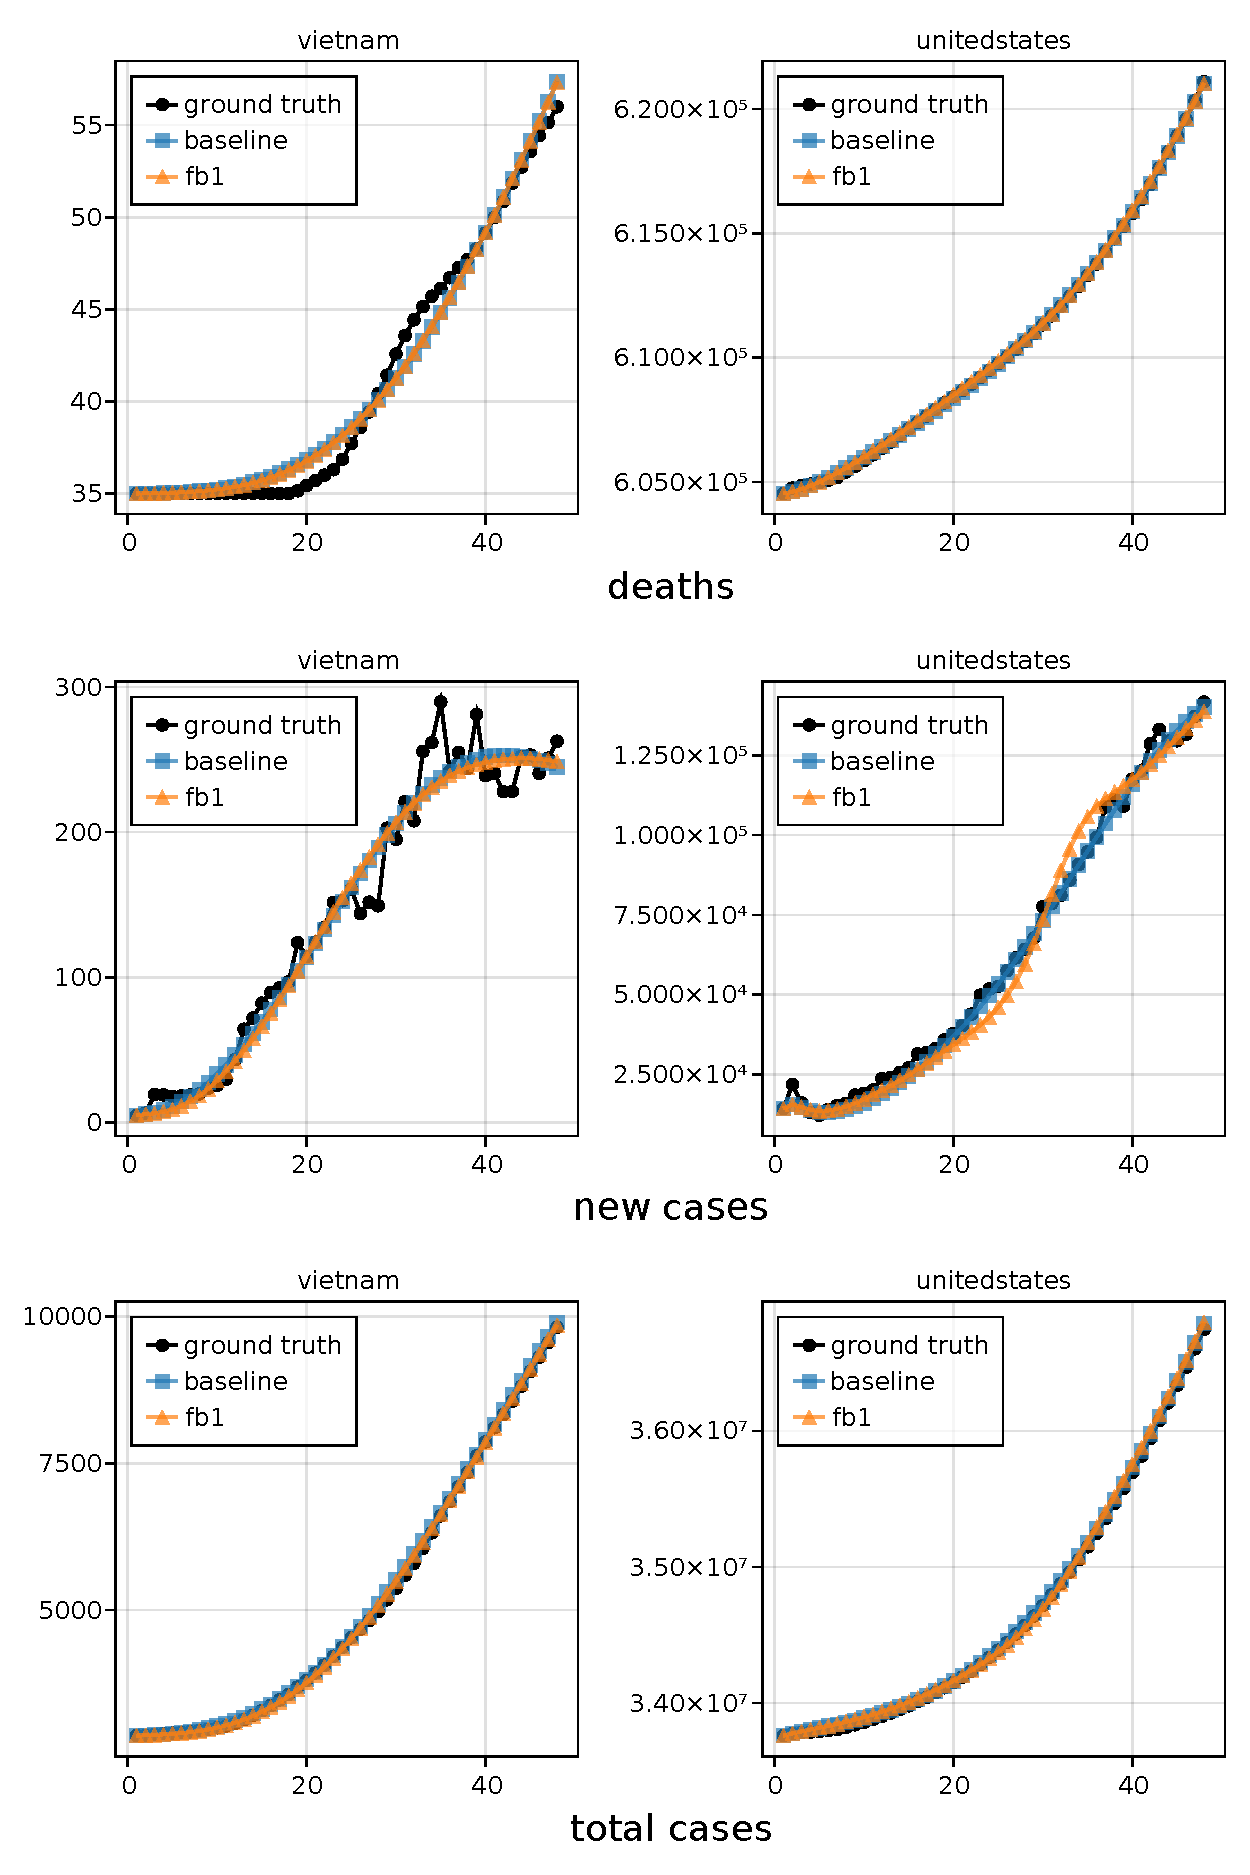
\includegraphics[scale=0.7]{fit_country_level.pdf}
    \caption{Predictions made by all versions of the model for the training period after having trained with country-level data. Each row contains the predictions for a compartment for each of the considered countries. Here the second version is denoted as \textit{fb1}}
    \label{fig:fit-country-level}
\end{figure}

\begin{figure}[!htb]
    \centering
    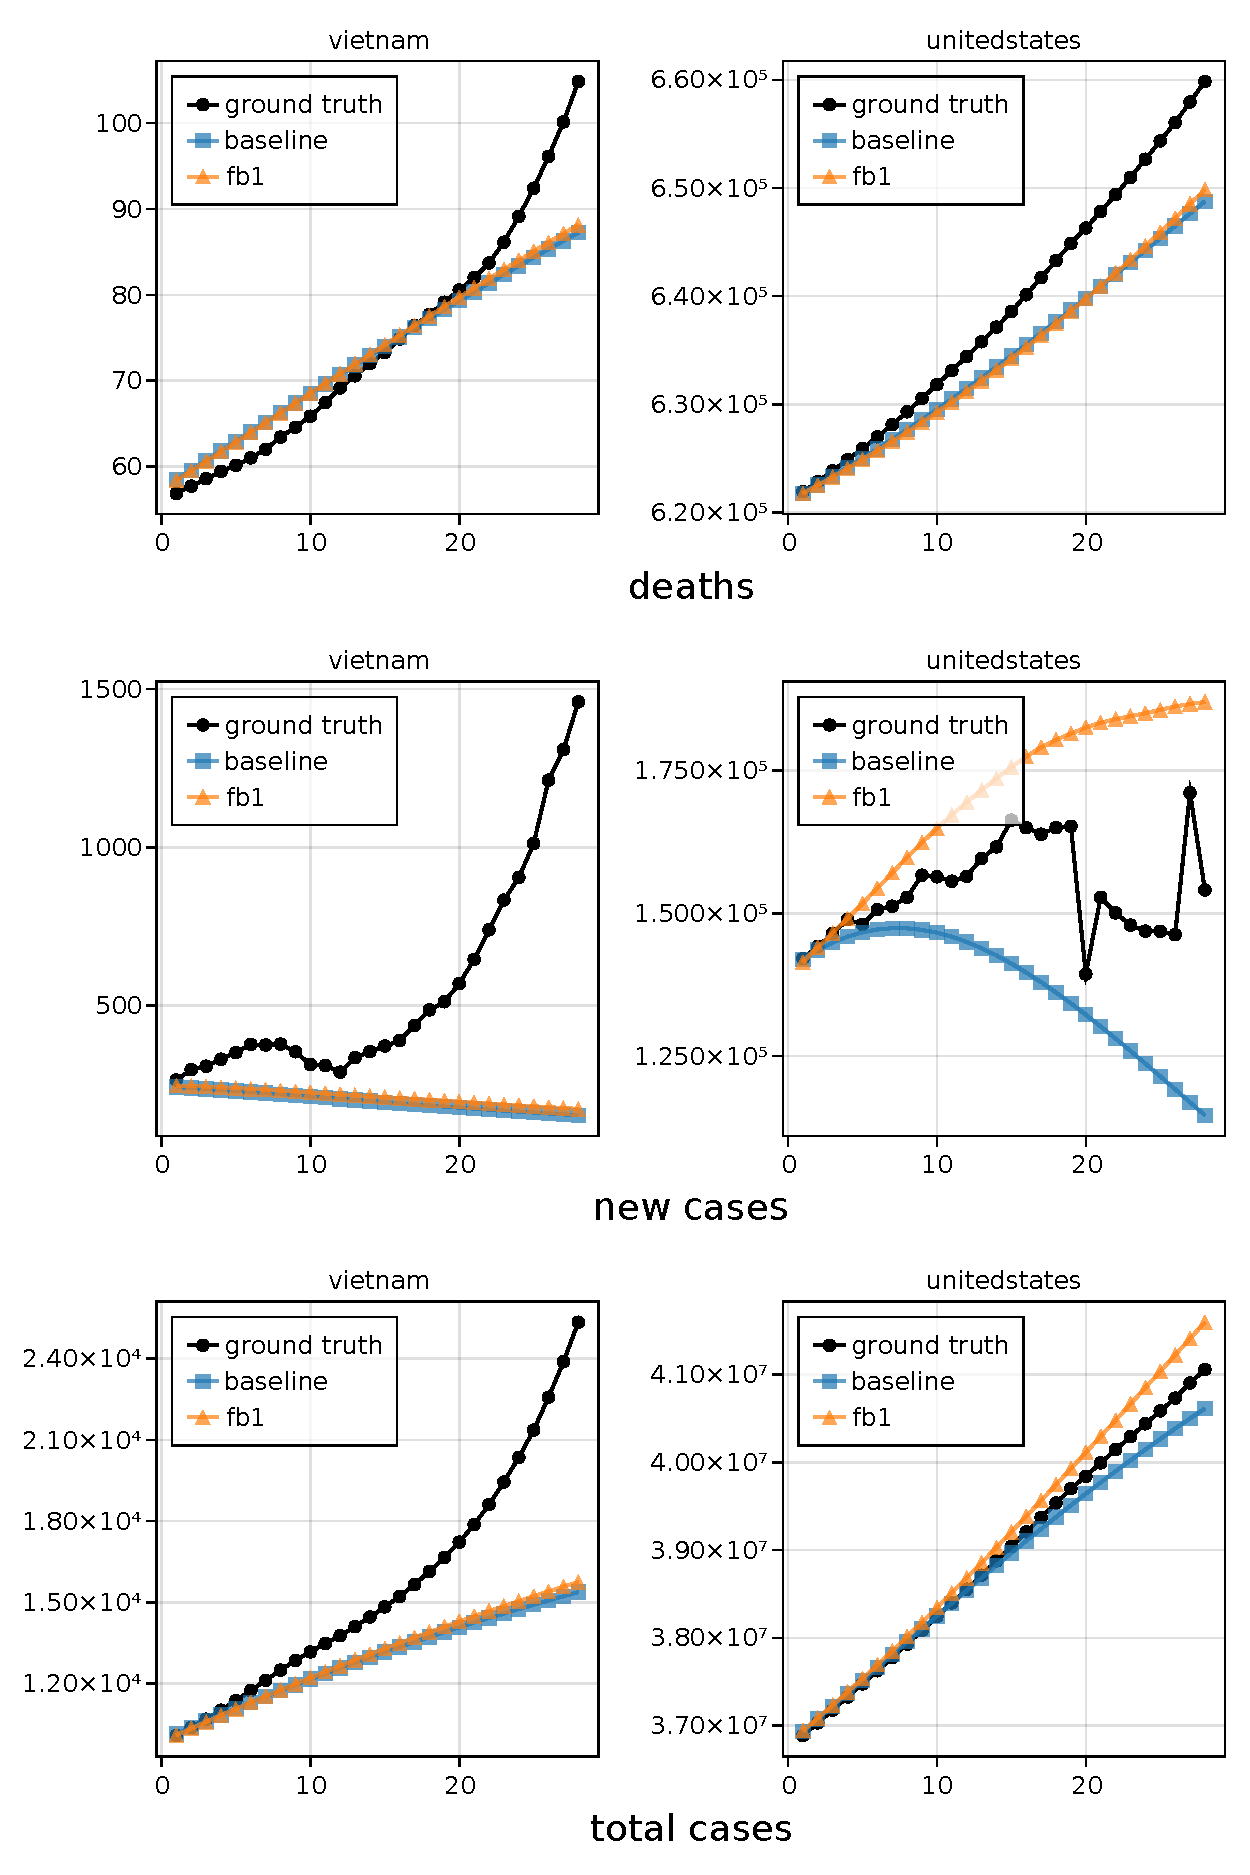
\includegraphics[scale=0.7]{pred_country_level.pdf}
    \caption{Predictions made by all versions of the model for the testing period after having trained with country-level data. Each row contains the predictions for a compartment for each of the considered countries. Here the second version is denoted as \textit{fb1}}
    \label{fig:pred-country-level}
\end{figure}

\begin{figure}[!htb]
    \centering
    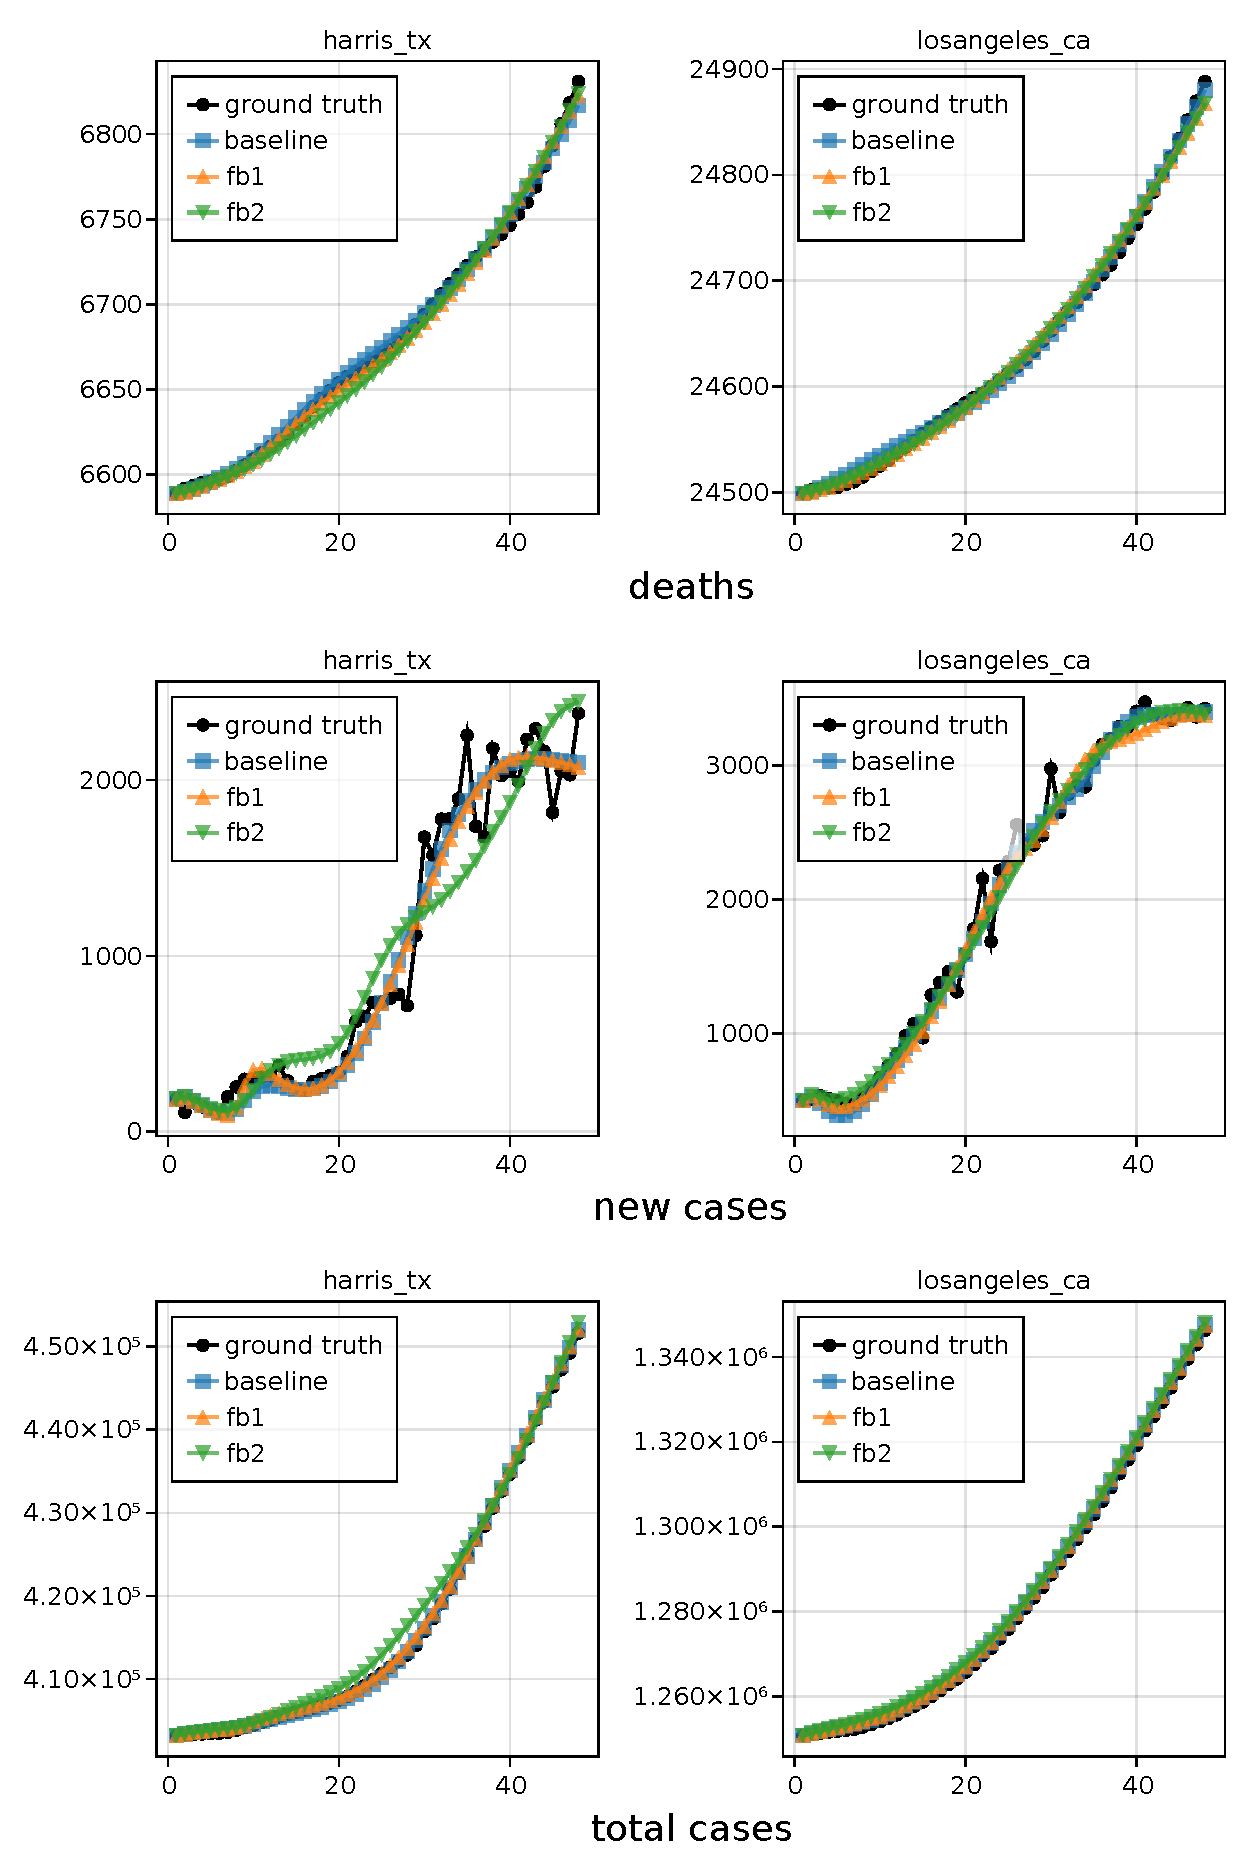
\includegraphics[scale=0.7]{fit_us_counties1.pdf}
    \caption{Predictions made by all versions of the model for the training period after having trained with data for Harris (Texas) and Los Angeles (California). Each row contains the predictions for a compartment for each of the considered counties. Here the second version is denoted as \textit{fb1} and the third version is denoted as \textit{fb2}}
    \label{fig:fit-us-counties1}
\end{figure}

\begin{figure}[!htb]
    \centering
    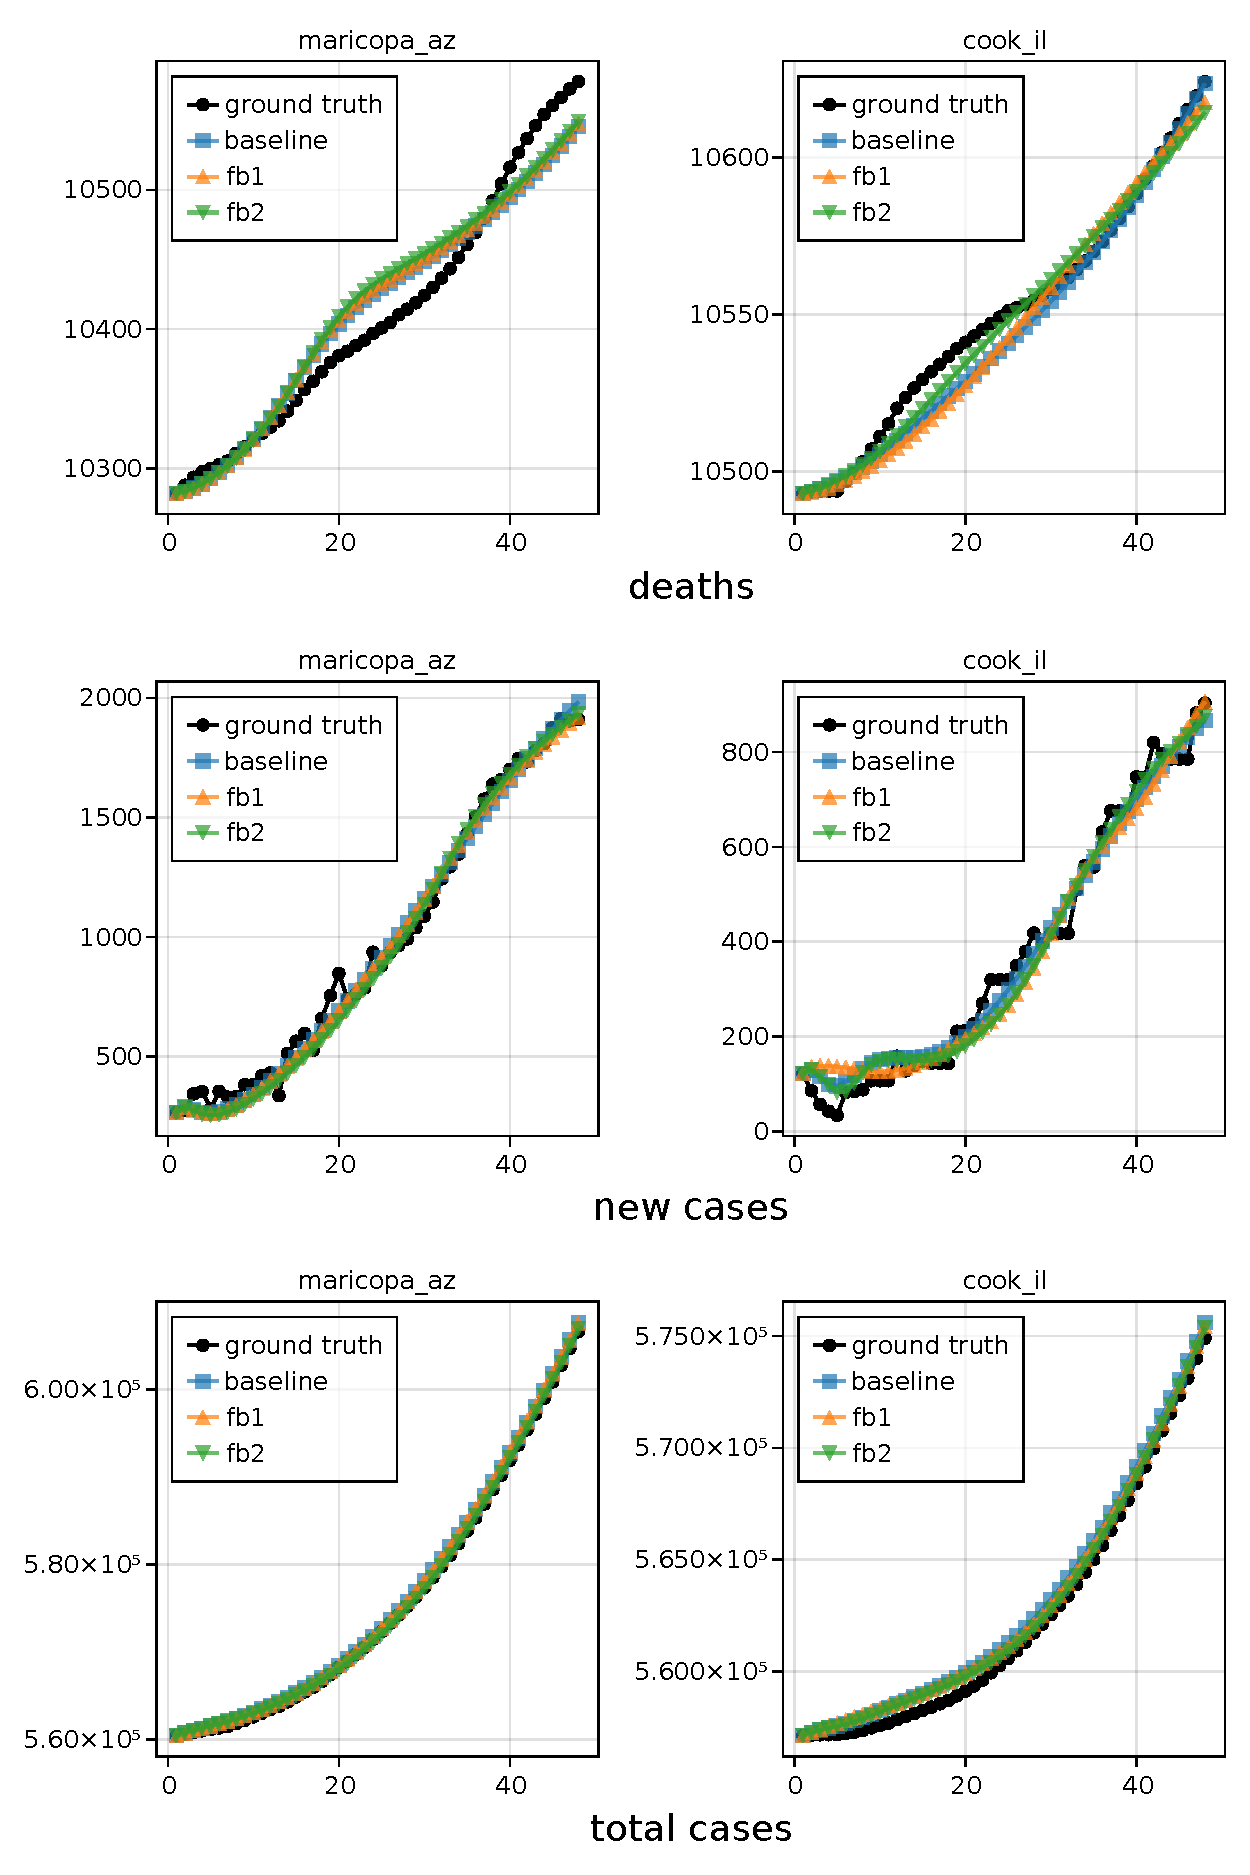
\includegraphics[scale=0.7]{fit_us_counties2.pdf}
    \caption{Predictions made by all versions of the model for the training period after having trained with data for Maricopa (Arizona) and Cook (Illinois). Each row contains the predictions for a compartment for each of the considered counties. Here the second version is denoted as \textit{fb1} and the third version is denoted as \textit{fb2}}
    \label{fig:fit-us-counties2}
\end{figure}

\begin{figure}[!htb]
    \centering
    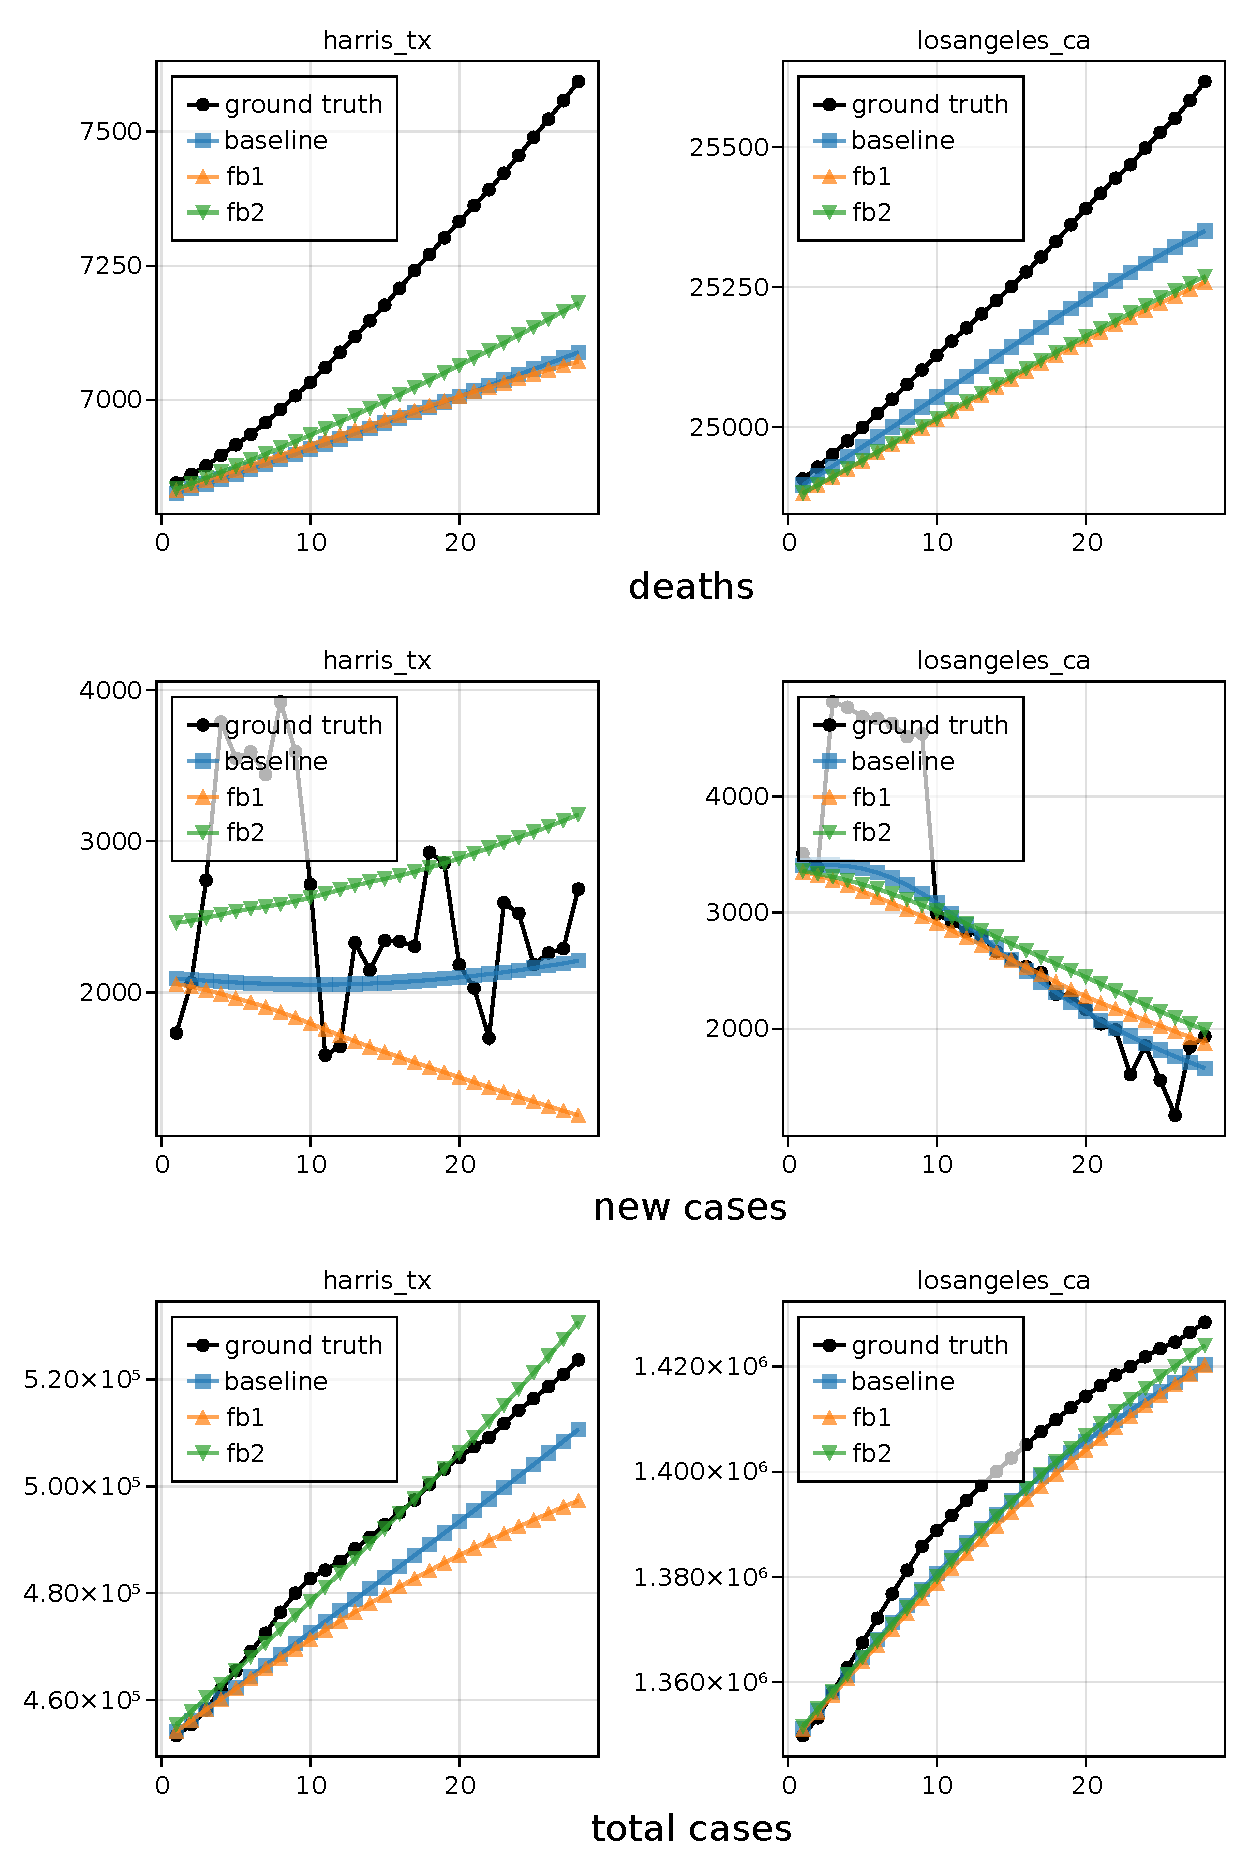
\includegraphics[scale=0.7]{pred_us_counties1.pdf}
    \caption{Predictions made by all versions of the model for the testing period after having trained with data for Harris (Texas) and Los Angeles (California). Each row contains the predictions for a compartment for each of the considered counties. Here the second version is denoted as \textit{fb1} and the third version is denoted as \textit{fb2}}
    \label{fig:pred-us-counties1}
\end{figure}

\begin{figure}[!htb]
    \centering
    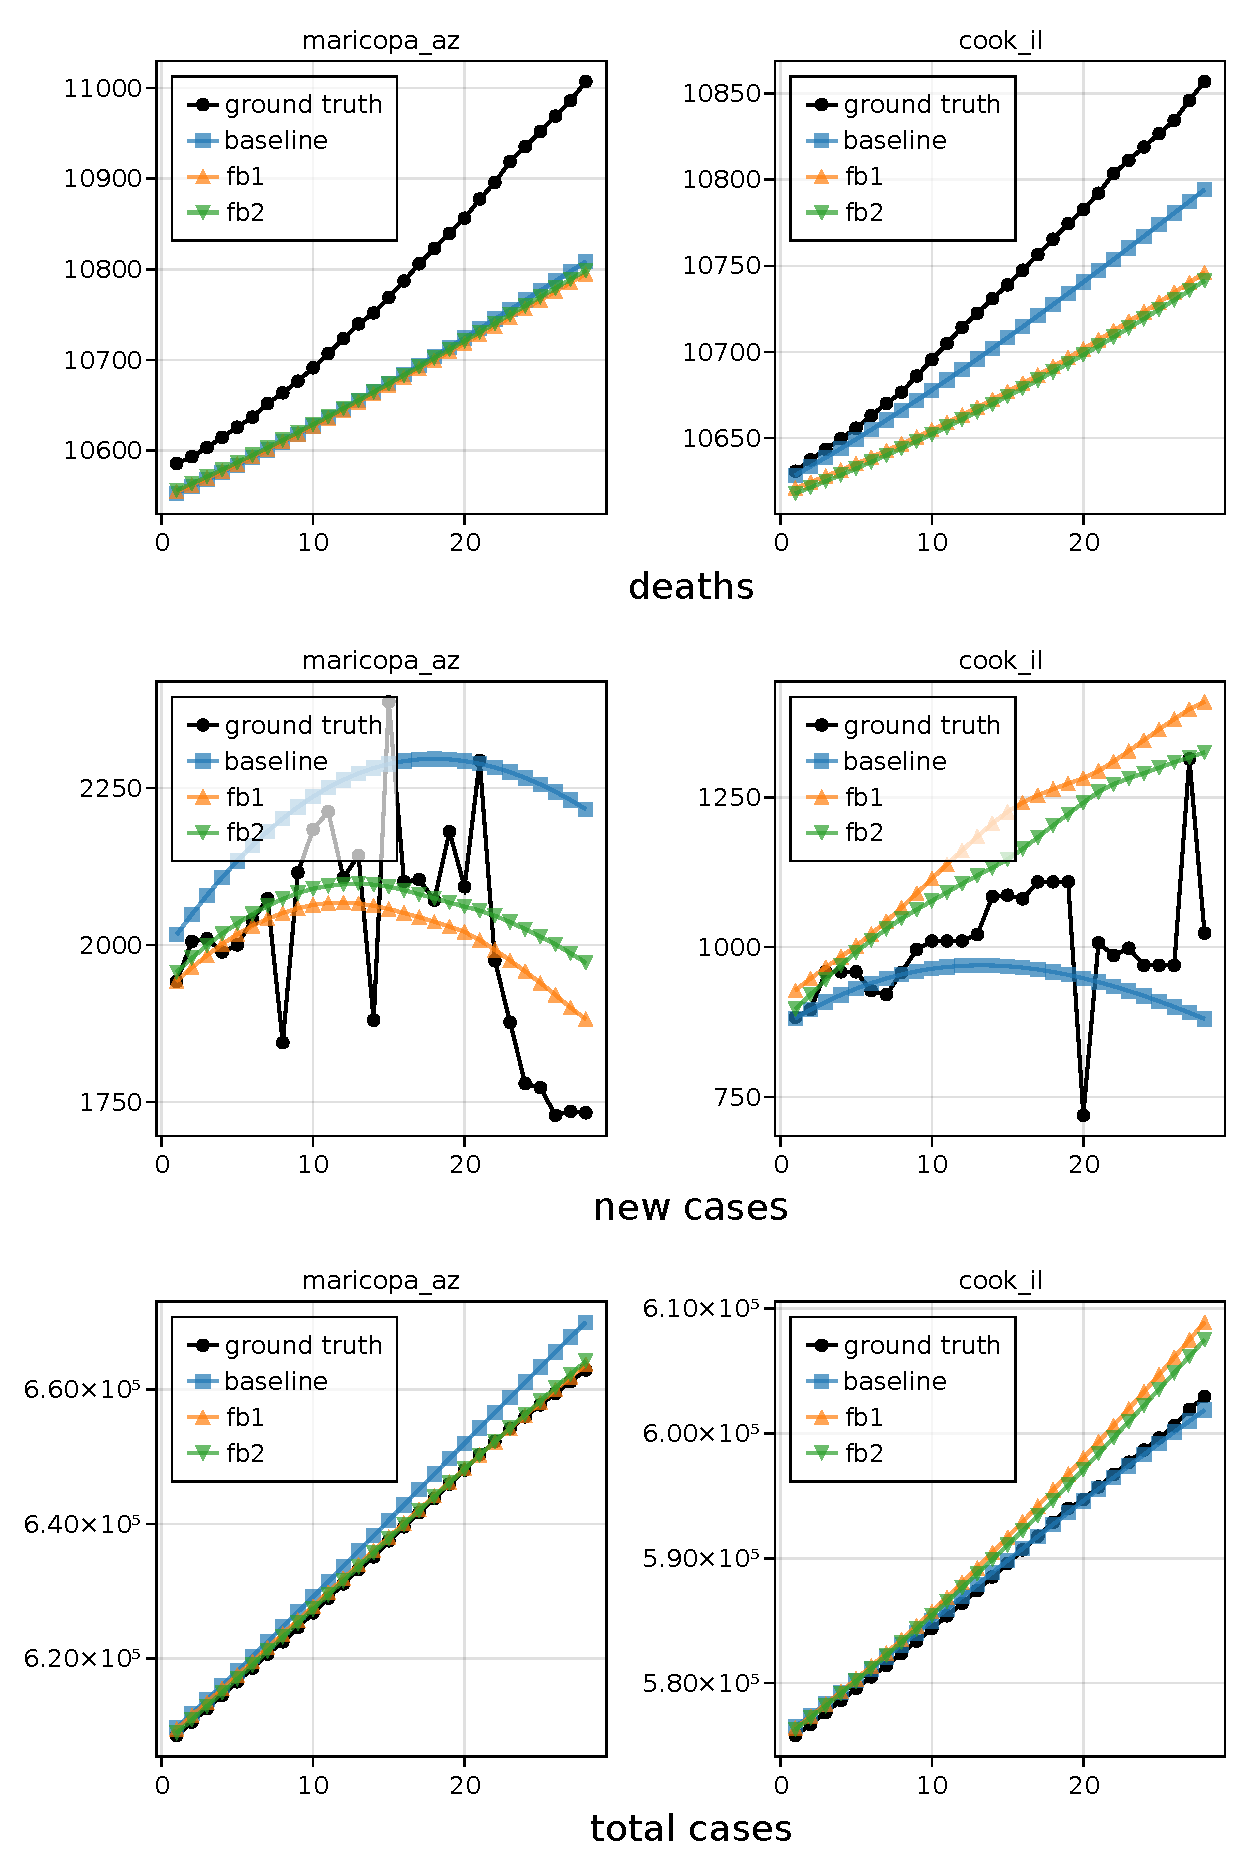
\includegraphics[scale=0.7]{pred_us_counties2.pdf}
    \caption{Predictions made by all versions of the model for the testing period after having trained with data for Maricopa (Arizona) and Cook (Illinois). Each row contains the predictions for a compartment for each of the considered counties. Here the second version is denoted as \textit{fb1} and the third version is denoted as \textit{fb2}}
    \label{fig:pred-us-counties2}
\end{figure}

\begin{figure}[!htb]
    \centering
    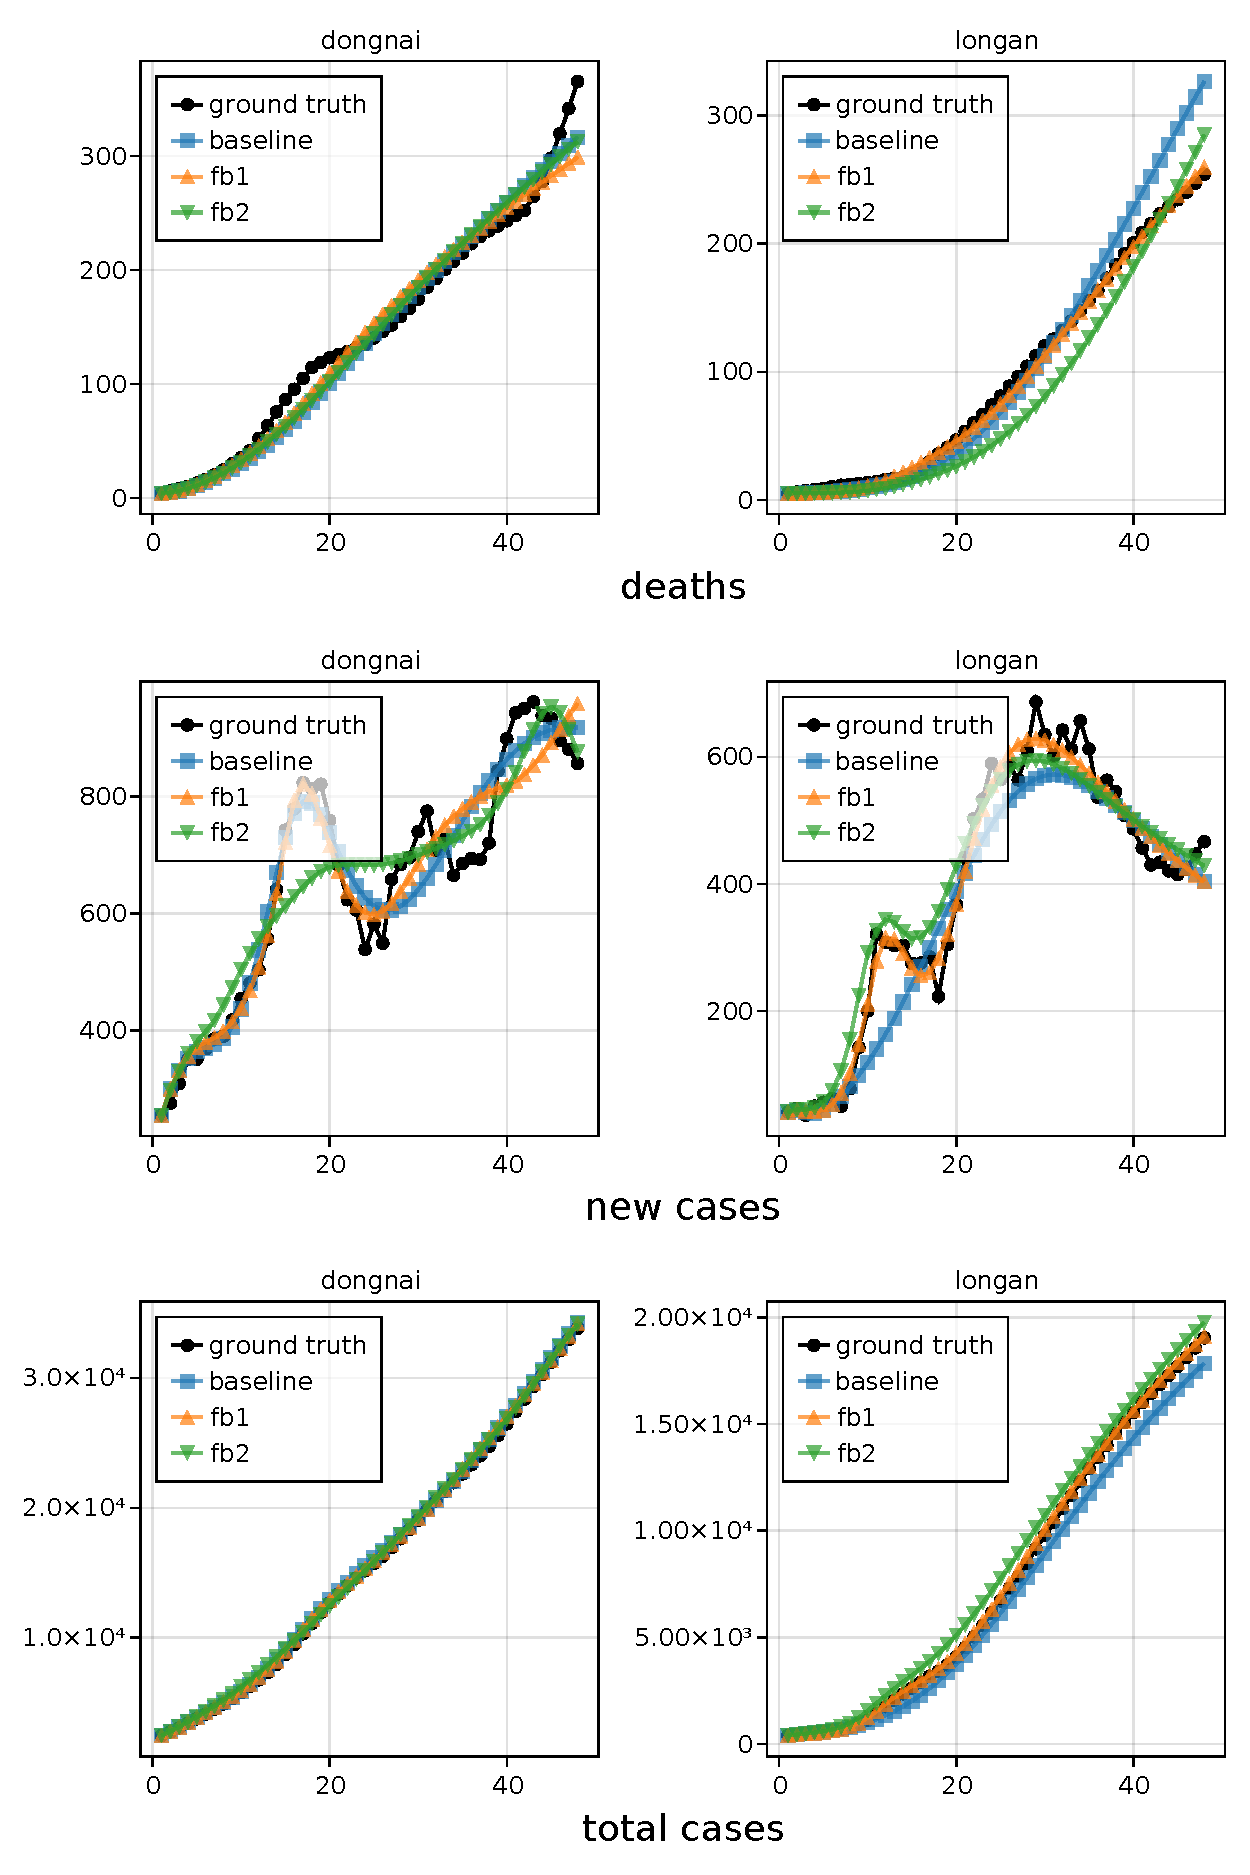
\includegraphics[scale=0.7]{fit_vn_provinces1.pdf}
    \caption{Predictions made by all versions of the model for the training period after having trained with data for Dong Nai and Long An. Each row contains the predictions for a compartment for each of the considered provinces. Here the second version is denoted as \textit{fb1} and the third version is denoted as \textit{fb2}}
    \label{fig:fit-vn-provinces1}
\end{figure}

\begin{figure}[!htb]
    \centering
    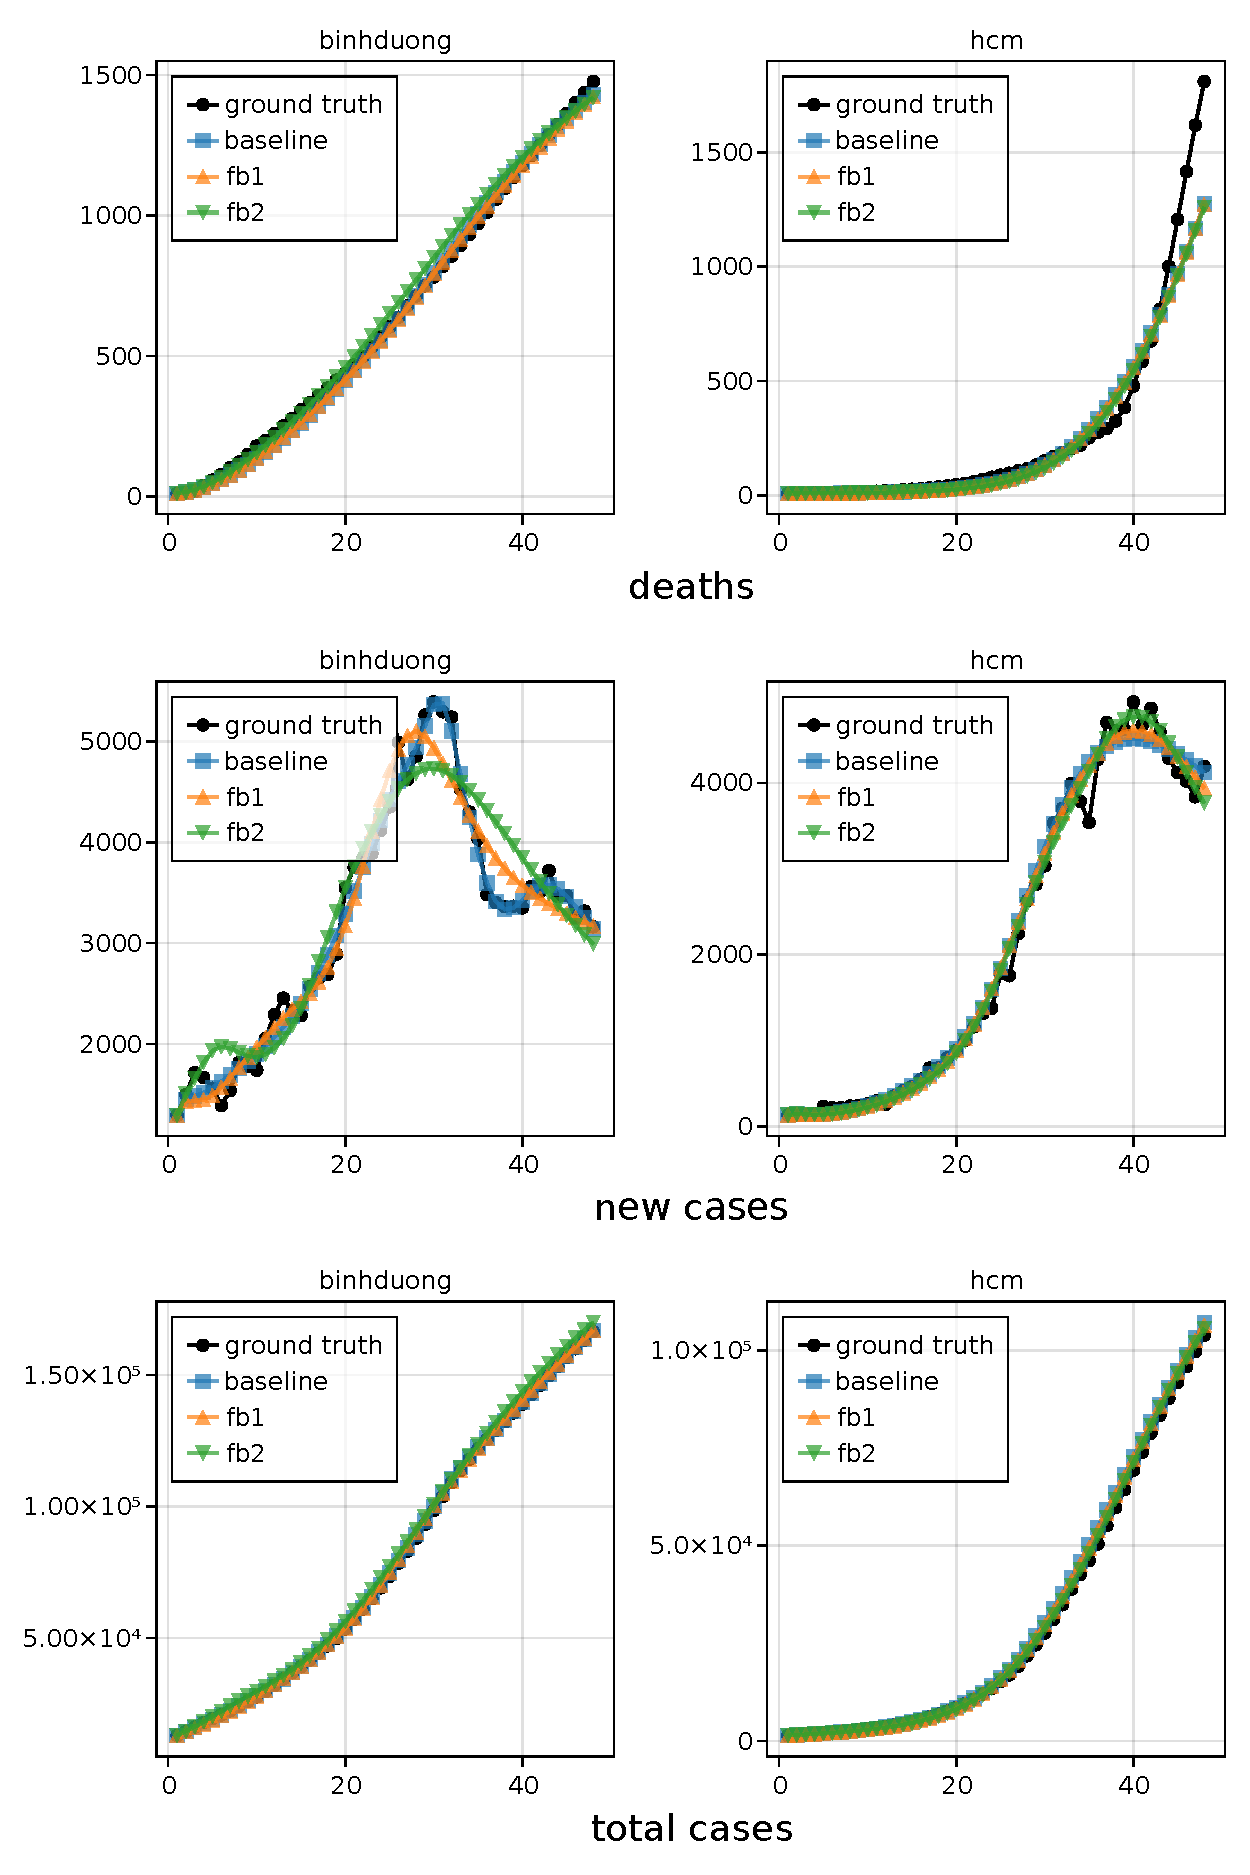
\includegraphics[scale=0.7]{fit_vn_provinces2.pdf}
    \caption{Predictions made by all versions of the model for the training period after having trained with data for Binh Duong and Ho Chi Minh city. Each row contains the predictions for a compartment for each of the considered provinces. Here the second version is denoted as \textit{fb1} and the third version is denoted as \textit{fb2}}
    \label{fig:fit-vn-provinces2}
\end{figure}

\begin{figure}[!htb]
    \centering
    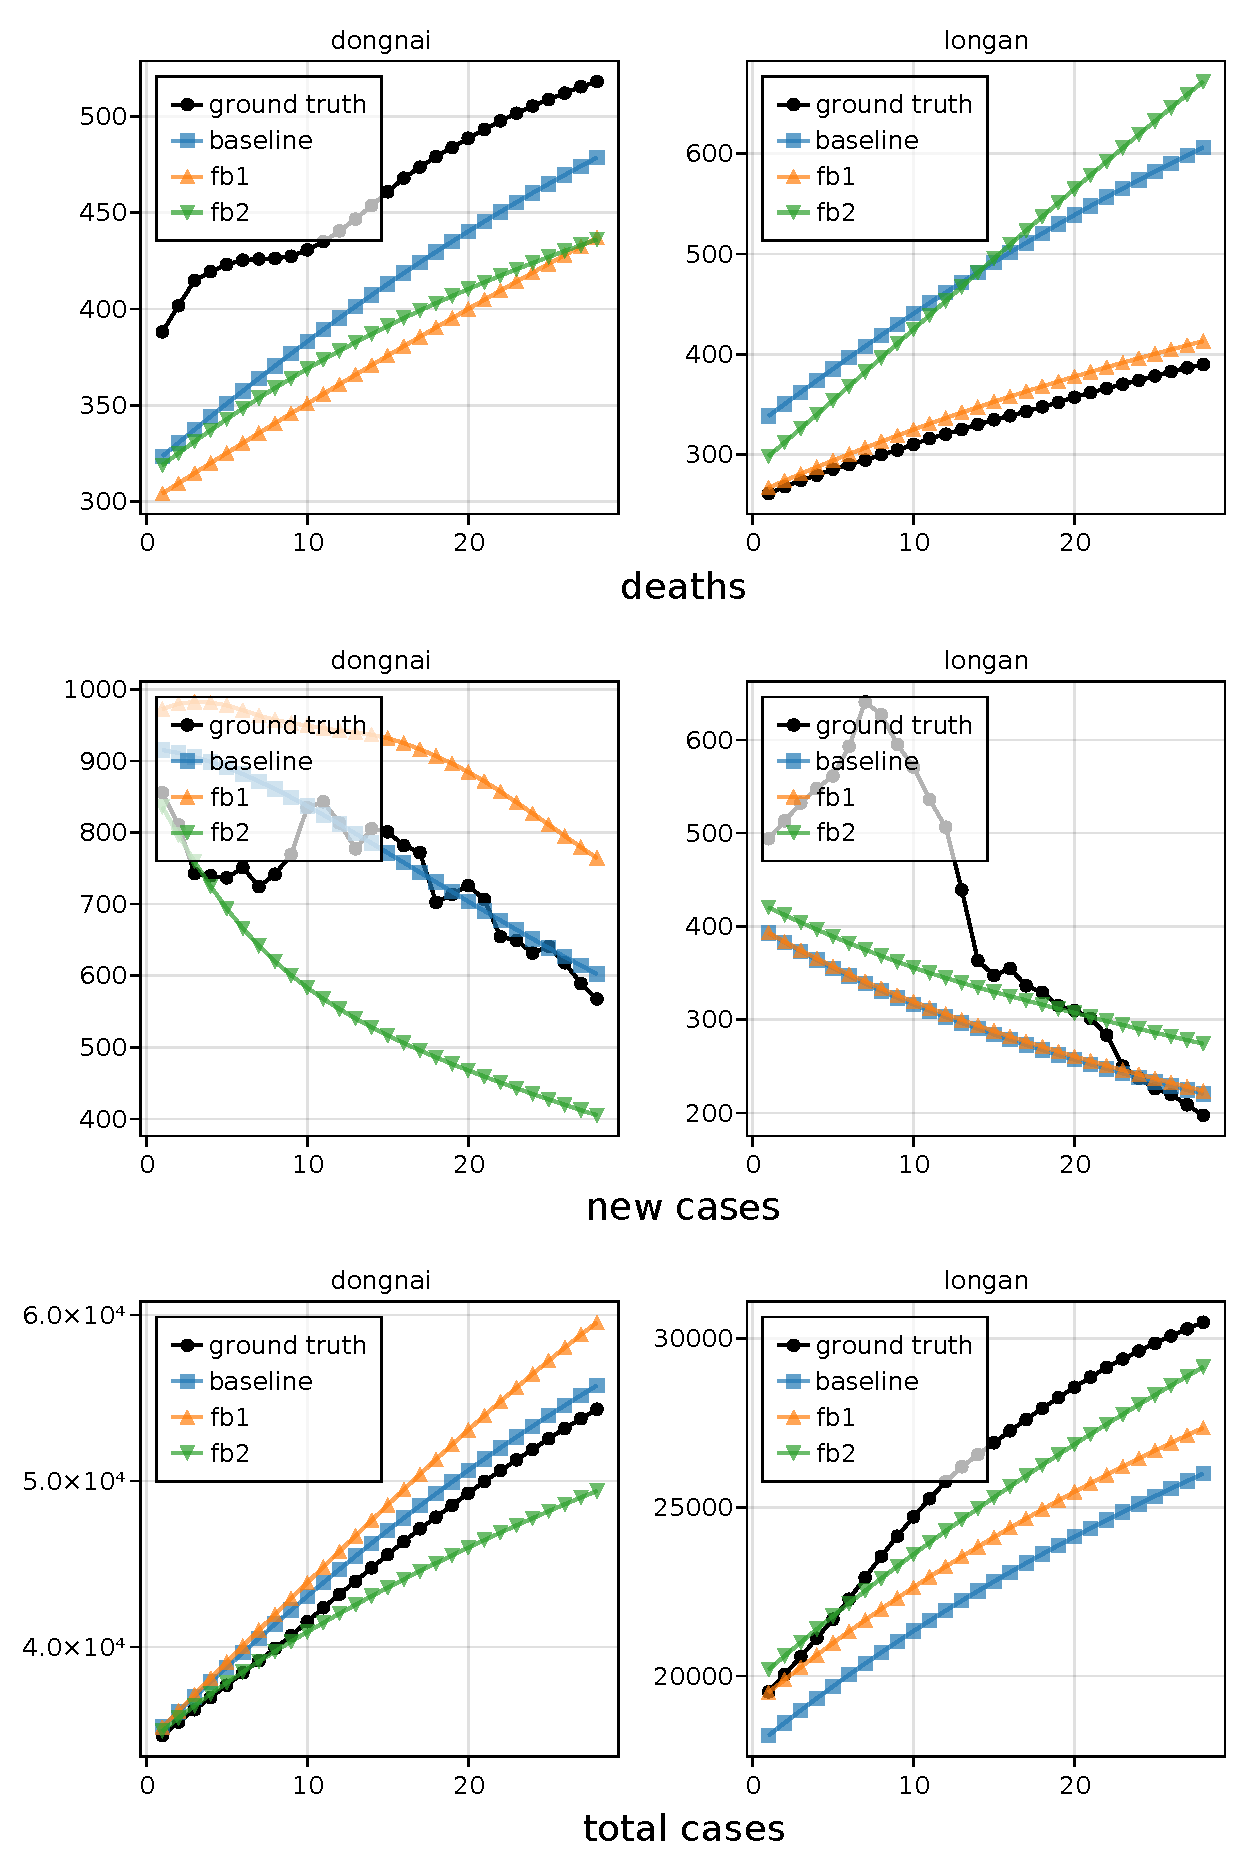
\includegraphics[scale=0.7]{pred_vn_provinces1.pdf}
    \caption{Predictions made by all versions of the model for the testing period after having trained with data for Dong Nai and Long An. Each row contains the predictions for a compartment for each of the considered provinces. Here the second version is denoted as \textit{fb1} and the third version is denoted as \textit{fb2}}
    \label{fig:pred-vn-provinces1}
\end{figure}


\begin{figure}[!htb]
    \centering
    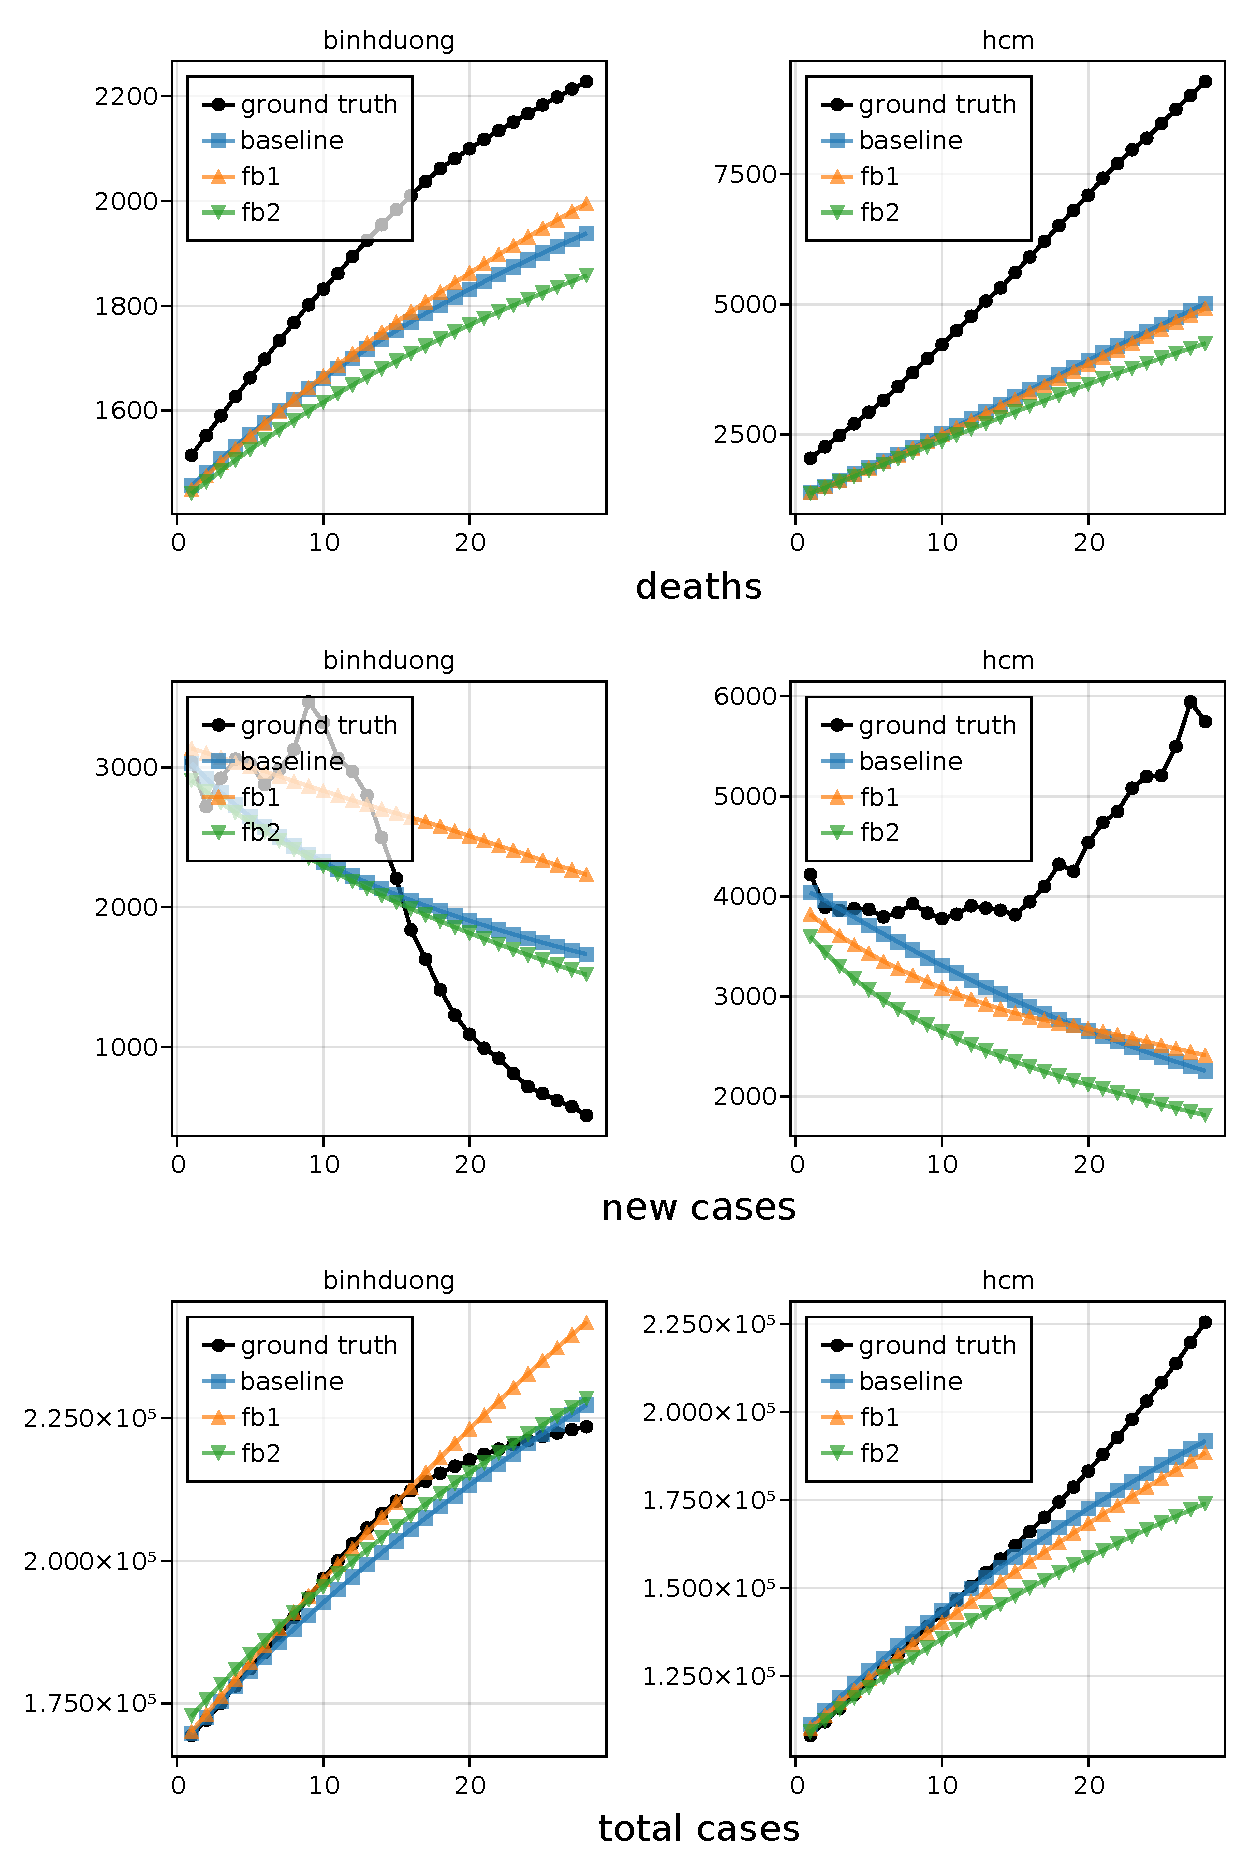
\includegraphics[scale=0.7]{pred_vn_provinces2.pdf}
    \caption{Predictions made by all versions of the model for the testing period after having trained with data for Binh Duong and Ho Chi Minh city. Each row contains the predictions for a compartment for each of the considered provinces. Here the second version is denoted as \textit{fb1} and the third version is denoted as \textit{fb2}}
    \label{fig:pred-vn-provinces2}
\end{figure}
